\documentclass[11pt, letterpaper]{article}

%% PAQUETES USADOS

\usepackage[left=3cm, right=3cm, top=1in, bottom=1in]{geometry}
\usepackage[spanish]{babel}
\usepackage{mathptmx}
\usepackage{graphicx}
\usepackage{svg}
\usepackage{csquotes}
\usepackage{dirtytalk}
\usepackage[most]{tcolorbox}
\usepackage[shortlabels]{enumitem}
\usepackage[style=ieee]{biblatex}
\usepackage{lipsum}

%% CONFIGURACIONES DEL PROYECTO

\addbibresource{../mylib.bib}

\newtheorem{definition}{Definición}

\newlist{syllabus}{enumerate}{10}
\setlist[syllabus]{label*=\arabic*., font=\bfseries, leftmargin=*}
\setlistdepth{10} 

%% ESTRUCTURA DEL DOCUMENTO

\begin{document}
\begin{titlepage}
    \centering
    {\bfseries \large 
    UNIVERSIDAD MAYOR DE SAN ANDRÉS - FACULTAD DE INGENIERÍA\par 
    INGENIERÍA 	ELECTRÓNICA
    }\\[2cm]
    
    
\includegraphics[width=0.2\textwidth]{assets/umsa.png}\\[1cm]
    
    {\LARGE \MakeUppercase{Perfil de Proyecto de Grado}}\\[1cm]
    
    \textbf{\Large \MakeUppercase{TUNKUNIA: Desarrollo de una librería “Open Source” para la implementación y seguimiento de trámites en Laravel. Caso de estudio: Sistema SIAI}}
    \vfill
    \MakeUppercase{Postulante: }
    \MakeUppercase{Ernesto Carlos Arena Alarcon}\\[1cm]
    
    \MakeUppercase{Asesor: }
    \MakeUppercase{Jorge Antonio Nava Amador}\\[1cm]
    
    \MakeUppercase{Docente D.A.M.: }
    \MakeUppercase{Jorge León}\\[1cm]
    
    \vfill
    {La Paz, \today\par}
\end{titlepage}
%%\begin{abstract}
\lipsum[1]
\end{abstract}
\clearpage
\tableofcontents
\newpage
\input{./introduction}
\section{Antecedentes}

\begin{tcolorbox}[breakable]
    
    Los antecedentes tienen que dar el origen que nos lleva a considerar el Problema
    que pretende ser resuelto por este proyecto. Introduce al mismo de forma
    algo más detallada que la introducción.
    Describe el escenario sobre el cual se desarrollará y mencionará qué se intentó para solucionarlo.
    
    Aquí puedo usar referencias al gobierno electrónico y las determinaciones
    del estado boliviano y de otras instituciones que suportean la idea de este
    proyecto.

    \begin{enumerate}
        \item Los trámites son importantes para el funcionamiento del estado
        \item Los gobiernos buscan digitalizarse
        \item Los gobiernos e instituciones prefieren software libre
        \item En Bolivia se hizo reglamentos
        \item Se adjudican obras para desarrollar software
        \item Se hizo el sistema SIAI con módulos de trámites
        \item Se hacen muchos desarrollos desde cero
        \item Existen librerías interesant
        \item Existe funcionalidad común 
        \item La reutilización de software es ventajosa
    \end{enumerate}
    
\end{tcolorbox}

Durante el desarrollo del sistema SIAI (Sistema de Información Ambiental
Industrial) del \say{Ministerio de Desarrollo Productivo y Economía Plural} por parte
de la empresa \say{2IES}, se pudo identificar ciertas funcionalidades comunes a muchos
sistemas de software gubernamentales, las cuales tienen que ver con los trámites, un proceso común en la administración pública de los gobiernos.

\subsection{El estado y el gobierno}

Si bien los temas filosóficos, históricos o políticos parecen carecer de
importancia en la presente propuesta, es importante entender el origen de la
problemática señalada más adelante desde la misma concepción del gobierno y del
estado, pues esto encaminará a entender su evolución, la cual eventualmente
origina la cuestión que se trata en este documento.

Para lo que nos atañe el estado es un fenómeno político que supuso
la separación o la salida de lo político del terreno social y \textbf{la
conversión del individuo en un ciudadano}, cuya relación de pertenencia
fundamental será con el estado al margen de cualquier característica particular
\cite{gordilloperezestadosurge}. Esto implica que el ciudadano tiene en adelante
una serie de obligaciones para con el estado al cual pertenece.

% κυβερνέιν

Por su lado, el gobierno (del griego
$\kappa \upsilon \beta \varepsilon \rho \nu \acute{\epsilon} \iota \nu$
kybernéin \textquote{pilotar un barco} o \textquote{capitán de un barco}), uno de los pilares del estado (Además del territorio, la población, la soberanía y el derecho), es un
sistema orgánico de autoridades a través del cual se expresa el poder del
Estado, creando, afirmando y desenvolviendo el orden jurídico
\cite{jorgefernandezruizdederecho}. Por lo tanto, es un actor que
funciona como cara del estado hacia la ciudadanía.

De esta manera, el gobierno es una entidad a la cual la ciudadanía se aproxima como figura de autoridad. Es quien, mediante sus distintos brazos de acción se encarga de administrar.

\subsection{Administración Pública: Interfaz ciudadano - gobierno}

La concepción de administración pública se remonta a muchos años atrás. Por
ejemplo, en el año 302 D.C. Claudio Mamertino ya hablaba del término
\say{administración de la cosa pública} (\textit{administratione res publicae})
\cite{nixonsaylorinpraiseroman}. Y es que está estrechamente relacionada con el
ejercicio del gobierno. Sin embargo, la aplicación y definición de la misma no
estaría clara hasta la llegada de Bonnin, el padre de la ciencia de la
administración pública.

Bonnin, en 1808, daba una definición primigenia sobre la administración pública:
\textquote{La que tiene la gestión de los asuntos comunes respecto al ciudadano
como miembro del estado} \cite{omarguerrerobonninsigloxxi}.

De este modo, la administración pública conecta al gobierno con la ciudadanía en
busca de beneficiar a esta última y la relaciona con el estado de forma más inmediata que entidades como el congreso.
Esta conexión se suele materializar en un procedimiento común, que es el
trámite.

\subsection{El trámite y la burocracia}

Poco se ha escrito estrictamente sobre los trámites a nivel académico. Sin
embargo, por conocimiento popular casi toda la sociedad sabe lo que son. Se sabe
también lo estrechamente relacionados que están con el gobierno, la burocracia y
el manejo de documentos.

La palabra trámite viene del latín \say{\textit{trames}},
\say{\textit{tramitis}}, que para los romanos significaba \say{senda},
\say{camino}, de donde se derivó el sentido actual de \say{vía legal o
procedimiento que debe seguir una gestión}. En inglés no existe una palabra que
tenga la traducción exacta de trámite, pero se usan distintas palabras como 
\say{\textit{Procedure}}, \say{\textit{Transaction}} o \say{\textit{Paperwork}}.
También en español se puede referir al mismo como \say{Procedimiento
administrativo}. En todas estas definiciones se tienen como común denominador
los términos: Proceso, Camino, Papeleo.

Los estados, para ejercer su poder mediante el gobierno, requieren de la
población cumplir con una serie de obligaciones, las cuales dieron paso al
surgimiento de diversas instituciones a las que acudimos a efecto de realizar
trámites.

Al respecto, de acuerdo a una definición del Gobierno de México en uno de sus
portales web se entiende como trámite a:

\begin{displayquote}
 Cualquier solicitud o entrega de información que las
personas físicas o morales del sector privado hacen ante una dependencia u
organismo descentralizado, ya sea para cumplir una obligación, obtener un
beneficio o servicio o, en general, a fin de que se emita una resolución, así
como cualquier documento que dichas personas estén obligadas a conservar
\cite{portalmexicotramite}.
\end{displayquote}

En el mismo portal se hace una clasificación de los trámites, donde se señalan 5
tipos de los mismos:

\begin{enumerate}
    \item De naturaleza obligatoria
    \item De beneficio
    \item De conservación
    \item De procedimiento
    \item De consulta
\end{enumerate}

Según la Real Academia de la Lengua Española, se define como \say{Cada uno de
los pasos y diligencias que hay que recorrer en un asunto hasta su conclusión}
\parencite{asaleDiccionarioLenguaEspanola}.

Los trámites constituyen además el conjunto de requisitos, pasos o acciones a
través de los cuales los individuos o las empresas piden o entregan información
a una entidad pública, con el fin de obtener un derecho o para cumplir con una
obligación \cite{rosethFinTramiteEterno2018}. A partir de esto, los distintos
trámites pueden tener algunas características distintas como poder ser gratuitos
o de pago o estar dirigido a sujetos específicos de la población (estar
condicionados).

Sin embargo, el proceso del trámite puede llegar a ser muy engorroso y
perjudicar a los ciudadanos. Tal es el caso de Domitila Murillo, quien debía
trasladarse entre varias ciudades de Bolivia para hacer largas filas y vagar
perdida entre una cantidad indefinida de requisitos. Cuando finalmente logró
recibir su cédula (el motivo del trámite), no le quedaron más que dos semanas
antes de fallecer \cite{charoskyquejatramite}

El caso de Domitila no es aislado, las distancias, la falta de definición de
requerimientos y la burocracia afectan al proceso del trámite. Los tiempos
suelen ser perjudiciales para la población, muchas veces llegando a tardar horas
por un simple trámite, como se puede ver en la figura \ref{fig:horastramite}.

\begin{figure}[htbp]
    \centering
    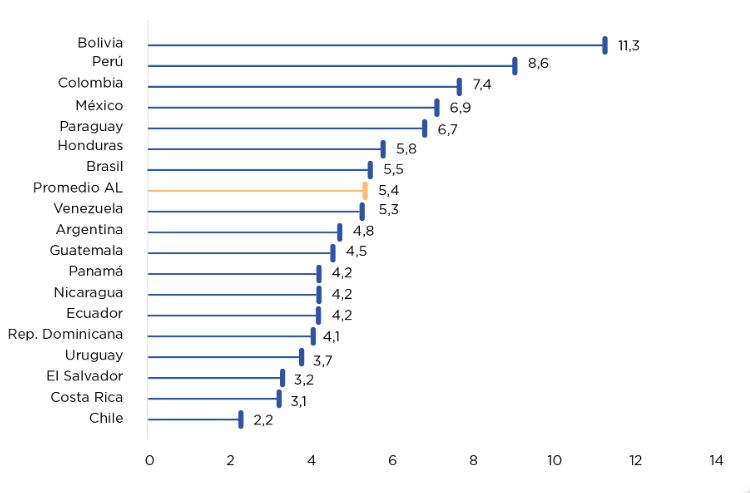
\includegraphics[width=0.7\textwidth]{assets/horastramite}
    \caption{Horas necesarias para completar un trámite, por país}{Fuente: Datos del Latinobarómetro, 2017}
    \label{fig:horastramite}
\end{figure}

El término burocracia se acuñó en el siglo 18 por el filósofo Francés Vincent de
Gournay, derivando del francés \textit{bureau} y \textit{cratie} que significan
\say{Escritorio para escribir} y \say{Gobierno} respectivamente
\cite{britannicabureaucracy}. Lo cual querría decir \say{Mandar desde el
escritorio}.

El sociólogo alemán Max Weber define burocracia como una forma racional de
organización que en su opinión es la forma más pura de sistema legal de
autoridad. La burocracia es según él, necesaria y algunas de sus características
fundamentales son las jerarquías, la especialización y la definición estricta
de reglas y regulaciones \cite{brajnikdictionaryofpublicadmin}.

Sin embargo, esta forma de organización suele tener como consecuencia en la
práctica una connotación negativa, ya que implica el consumo de mayores tiempos
de ejecución para distintas tareas administrativas, como es el caso del trámite.
Una tendencia reciente cree que el uso de las tecnologías de la información
podrían ayudar a mitigar este problema.

\subsection{En busca del \textit{e-government}}

En una entrevista a Carlos Jiménez, responsable mundial de \textit{IEEE e-government}, el mismo señala que el gobierno electrónico es una fase para llegar a tener gobiernos inteligentes y abiertos y que consiste en implantar la tecnología para mejorar procesos administrativos y permitir la interacción con los ciudadanos.

Si bien lo anterior nos puede dar una idea sobre lo que es el Gobierno Electrónico, se debe notar que no existe consenso en su definición y que más de una vez el término se usa de forma indistinta con \say{Gobierno Digital} o incluso algunas veces con \say{Gobierno Inteligente}. Sin embargo, un factor común es el uso de tecnologías de la información dentro del gobierno, como veremos a continuación.

Las siguientes son algunas definiciones:

Según el Gobierno de México: El concepto de Gobierno Electrónico incluye todas aquellas actividades basadas en las modernas tecnologías informáticas, en particular Internet, que el Estado desarrolla para aumentar la eficiencia de la gestión pública, mejorar los servicios ofrecidos a los ciudadanos y proveer a las acciones de gobierno de un marco mucho más transparente que el actual.

Por su lado, el Gobierno de Bolivia define Gobierno Electrónico como: la aplicación de las tecnologías de la información y la comunicación (TIC) al funcionamiento del sector público, con el objeto de incrementar la eficiencia, la transparencia y la participación ciudadana.
Engloba la interacción digital entre el estado y los ciudadanos, entre entidades públicas, el Estado y los servidores públicos y, entre el Estado y las empresas, contribuyendo al uso intensivo de las TIC.

El Banco Mundial lo define como \say{El uso de las tecnologías de la información y comunicaciones para mejorar la eficiencia, la efectividad, la transparencia y la rendición de cuentas del gobierno}.

Las Naciones Unidas, por su lado, lo definen como \say{La utilización de Internet y la \textit{World Wide Web} para entregar información y servicios del gobierno a los ciudadanos}.

El elemento clave en estas definiciones es la \say{gestión pública por medios digitales}.

Muchos países han visto la transformación hacia el gobierno electrónico como una prioridad en los últimos años y para lograrlo han implementado políticas públicas y una serie de estrategias.

Si bien, el Gobierno Abierto no está necesariamente relacionado al Gobierno Electrónico, en la práctica se ha visto cómo ambos conceptos actúan de forma estrecha gracias al uso de las TIC. El Gobierno Abierto surge por la creencia que el acceso a la información de gobierno por parte de los ciudadanos es un derecho esencial que fortalece el ejercicio democrático \cite[13]{naserGobiernoElectronicoGestion2011}.

Dada la importancia que tiene la implementación del gobierno electrónico tanto para el estado como para la población, las Naciones Unidas realizan un reporte sobre los avances en la misma. Uno de los índices empleados es el \textit{EGDI (e-Government Development Index)}, que es un indicador importante y que nos permite ver la pronta adopción de políticas que favorecen la implementación del gobierno electrónico. Esto se puede ver reflejado en la figura \ref{fig:egdi2020_2022}, que compara la situación del indicador entre 2020 y 2022.

\begin{figure}[!h]
    \centering
    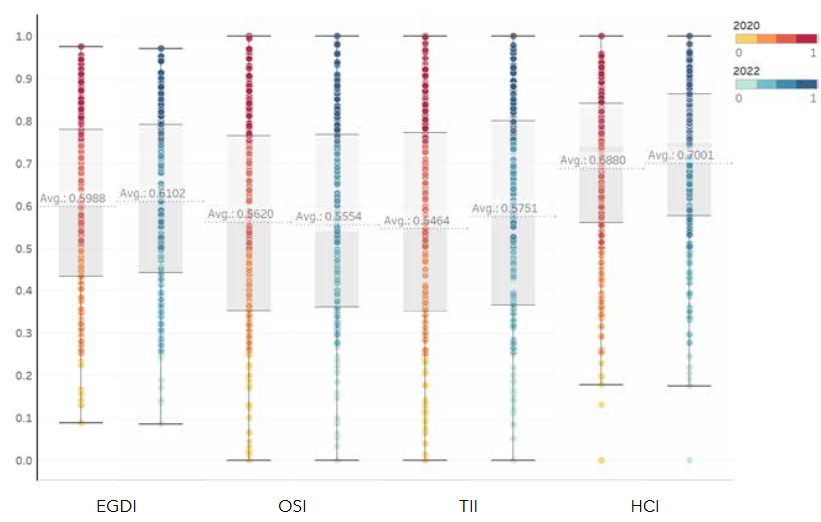
\includegraphics[width=0.7\textwidth]{assets/egdi2020_2022}
    \caption{Valores promedio del EGDI y sus componentes}{Fuente: 2020 and 2022 United Nations E-Government Surveys}
    \label{fig:egdi2020_2022}
\end{figure}

El Gobierno Electrónico brinda muchos beneficios a la población como la eliminación de barreras temporales y espaciales, acceso igualitario a la información, colaboración, aumento en la producción de bienes y servicios, en suma, brinda mayor calidad de vida a la ciudadanía.

Los beneficios se crean sobre cuatro actores: Gobierno, Empresas, Ciudadanos y Empleados. Generando cuatro tipos de relaciones (figura \ref{fig:g2all}):

\begin{enumerate}
    \item G2C: Government to Citizen
    \item G2B: Government to Business
    \item G2E: Government to Employee
    \item G2G: Government to Government
\end{enumerate}

\begin{figure}[!h]
    \centering
    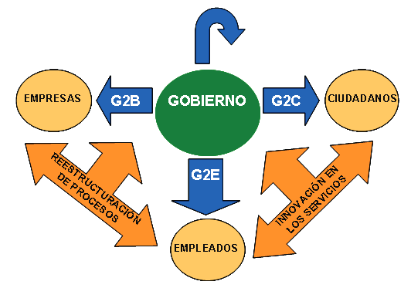
\includegraphics[width=0.7\textwidth]{assets/g2all}
    \caption{Modelo Relacional de Servicios de la Administración Pública}{Fuente: Naser, El Gobierno Electrónico}
    \label{fig:g2all}
\end{figure}

\subsection{FLOSS: Herramientas de libertad}

\subsection{Esfuerzos en Bolivia y la región}

\subsection{Sistema SIAI}

\subsection{RAI, IAA, DIA: Un caso común}

\subsection{Componentes de Software Reutilizables}


\subsection{Software Libre Reutilizable}

la creación del \textit{Sofware FOSS} se atribuye a Richard Stallman, conocido como el padre del código abierto. El mismo creía que todos merecían colaborar libre y abiertamente con otros utilizando software, por lo que en 1983 presentó el Proyecto GNU, el cual constituye el primer sistema operativo libre. Posteriormente en 1985 siguió con la creación de la Free Software Foundation para apoyar aún más a la comunidad del software libre. A finales de la década de 1990 el reconocimiento generalizado de Linux y el lanzamiento del código fuente del navegador \textit{Netscape} aumentó el interés y la participación en el Software libre. La etiqueta de \textit{Open Source} se creó en una sesión estratégica celebrada el 3 de febrero de 1998 en Palo Alto, California, poco después de que se publicara el código fuente de \textit{Netscape}. Sin embargo, el término que actualmente se considera más correcto de usar es el de \textit{FOSS}, ya que acuña ambas definiciones \textit{(Free and Open Source Software)}. 

El software libre es principalmente colaborativo y reutilizable, afectando positivamente a la economía. En un principio, las grandes corporaciones se negaban a apoyar el desarrollo de \textit{FOSS}. Sin embargo, vista la utilidad del mismo, hoy en día se prefiere su utilización.

El software que se reutiliza es software de mayor calidad y a menores costos económicos y temporales. Implica una gran ventaja sobre los desarrollos desde cero.
\section{Situación Actual}

En la actualidad podemos encontrar diversos intentos de modernizar los procesos administrativos de entidades públicas y podemos tomar sus experiencias como inspiración para la realización de una herramienta reutilizable de software. Además, existen paquetes de software que, aunque de manera indirecta, pueden ayudar en la creación de trámites.

\subsection{Sistemas realizados para el control de trámites}

Sólo en Latinoamérica, cada país reportó mediante las autoridades de gobierno electrónico tener entre 1000 y 5000 trámites diferentes. Esto implica que ya hubo muchos esfuerzos para crear sistemas que digitalicen esta actividad. A continuación se listan algunos.

\subsubsection{A nivel académico}

Podemos encontrar una gran cantidad de proyectos de grado realizados en la región que tratan sobre la implementación de sistemas de control de trámites:

\begin{itemize}
    \item SISTEMA DE CONTROL DE TRÁMITES UTILIZANDO MAQUINAS DE TURING CASO: DIVISIÓN DE GESTIONES ADMISIONES Y REGISTROS U.M.S.A.
    \item Desarrollo e Implementación del Sistema de Tramite
          Documentario en la Municipalidad Provincial de
          Huancayo para la atencion de expedientes.
    \item DESARROLLO DE UN SISTEMA WEB PARA MEJORAR  EL PROCESO DE TRÁMITE DOCUMENTARIO ADMINISTRATIVO DEL HOSPITAL SUB REGIONAL DE  ANDAHUAYLAS
    \item Sistema de información de trámite documentario basado en tecnología web para institutos de educación superior tecnológicos de la región Ancash en el año 2016
    \item Programa de automatización de los procedimientos de trámite documentario en la calidad del servicio a los usuarios del Hospital Nacional Arzobispo Loayza – Lima, 2016
    \item Implementación de un sistema de trámite documentario para la Agencia de Compras de las Fuerzas Armadas
    \item Implementación De Un Módulo De Control Y Seguimiento Para Mejorar La Gestión Del Trámite Documentario En La Municipalidad Distrital De Cayaltí, 2018
    \item Desarrollo de una aplicación web responsive para mejorar el proceso de trámite documentario en un colegio profesional
    \item Desarrollar un sistema web de trámite documental para mantener las acreditadoras de la escuela de ingeniería informática de la URP
\end{itemize}

De estos trabajos podemos destacar dos por su relevancia con el proyecto que se propone en este documento:

\paragraph{SISTEMA DE CONTROL DE TRÁMITES UTILIZANDO MAQUINAS DE TURING CASO: DIVISIÓN DE GESTIONES ADMISIONES Y REGISTROS U.M.S.A.}

En este proyecto de grado, realizado el año 2007, se toma como enfoque teórico a las máquinas de Turing. En dichas máquinas, que son un modelo matemático de computación, se describe una suerte de cinta dividida en casillas que funciona como memoria y un cabezal que escribe y lee de esa cinta, cambiando de estados. Esta conceptualización, sin ser estrictamente especificada se puede ver repetida en otras implementaciones de módulos de control de trámites.

\paragraph{Implementación De Un Módulo De Control Y Seguimiento Para Mejorar La Gestión Del Trámite Documentario En La Municipalidad Distrital De Cayaltí}

Esta tesis busca demostrar la importancia de la creación de un módulo específico de trámites que sea reutilizable. Brinda algunas recomendaciones sobre su implementación, pero no realiza ninguna implementación práctica.

\subsubsection{A nivel comercial}

Si bien, no existen módulos de trámite que se puedan integrar en sistemas más grandes de manera comercial, sí se puede ver sistemas completos con la funcionalidad de gestión de trámites que ofrecen todo lo necesario para llevar a cabo procesos administrativos. Algunos son:

\begin{itemize}
    \item SoftExpert - Gestión de Trámites: Visibilidad y control sobre el procesamiento de documentos, archivos y objetos
    \item R2 Docuo: Expedientes, Solicitudes y trámites a toda velocidad: En su homepage puede verse la funcionalidad de seguimiento temporal de trámites (figura \ref{fig:r2docuotimeline})
    \item Filestage: Si bien no es específico para trámites, tiene un sistema de tránsito de documentos hasta su aceptación, que es una funcionalidad común en los trámites.
\end{itemize}

\begin{figure}[!h]
    \centering
    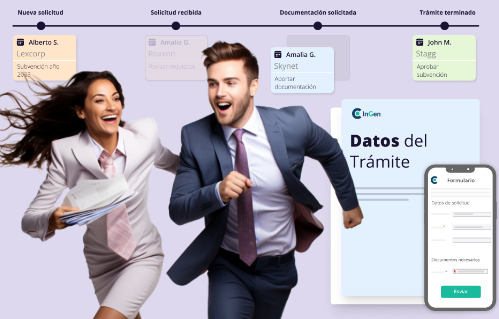
\includegraphics[width=0.7\textwidth]{assets/r2docuotimeline}
    \caption{Captura del homepage de R2 Docuo donde se puede ver el timeline de un trámite}{Fuente: https://www.r2docuo.com/es/expedientes-y-tramites}
    \label{fig:r2docuotimeline}
\end{figure}

Se debe notar que si bien los dos primeros logran la funcionalidad deseada en este proyecto, no permiten la personalización, no son necesariamente software libre y no se pueden introducir en sistemas más grandes de la misma manera que lo haría un paquete de software reutilizable.

\subsection*{Paquetes de software que facilitan la creación de módulos de trámites}

La cantidad de paquetes de software que existen y que se puede considerar que ayudan en el proceso de gestión, control y seguimiento de trámites es abundante, por lo que nos centraremos en aquellas presentes en el ecosistema de Laravel.

El seguimiento de trámites requiere que tengamos guardada la información de todos los pasos de un trámite y los cambios realizados. Además, la naturaleza de los trámites, como se podrá ver en el análisis de la solución, tiene que ver con estados (pasos de un procedimiento administrativo). Es por esto que las siguientes librerías podrían ser utilizadas con un objetivo similar al paquete que se pretende desarrollar en este proyecto:

\begin{itemize}
    \item Laravel Auditing: Permite mantener control sobre los datos en una aplicación y para hacer seguimiento de los cambios realizados en los mismos. Es muy potente y fácil de usar.
    \item Laravel Eloquent State Machines: Máquinas de estado aplicadas sobre los modelos Eloquent (figura \ref{fig:laravelstatemachines}).
    \item Laravel-Permission: Permite asociar usuarios con roles.
\end{itemize}

\begin{figure}[!h]
    \centering
    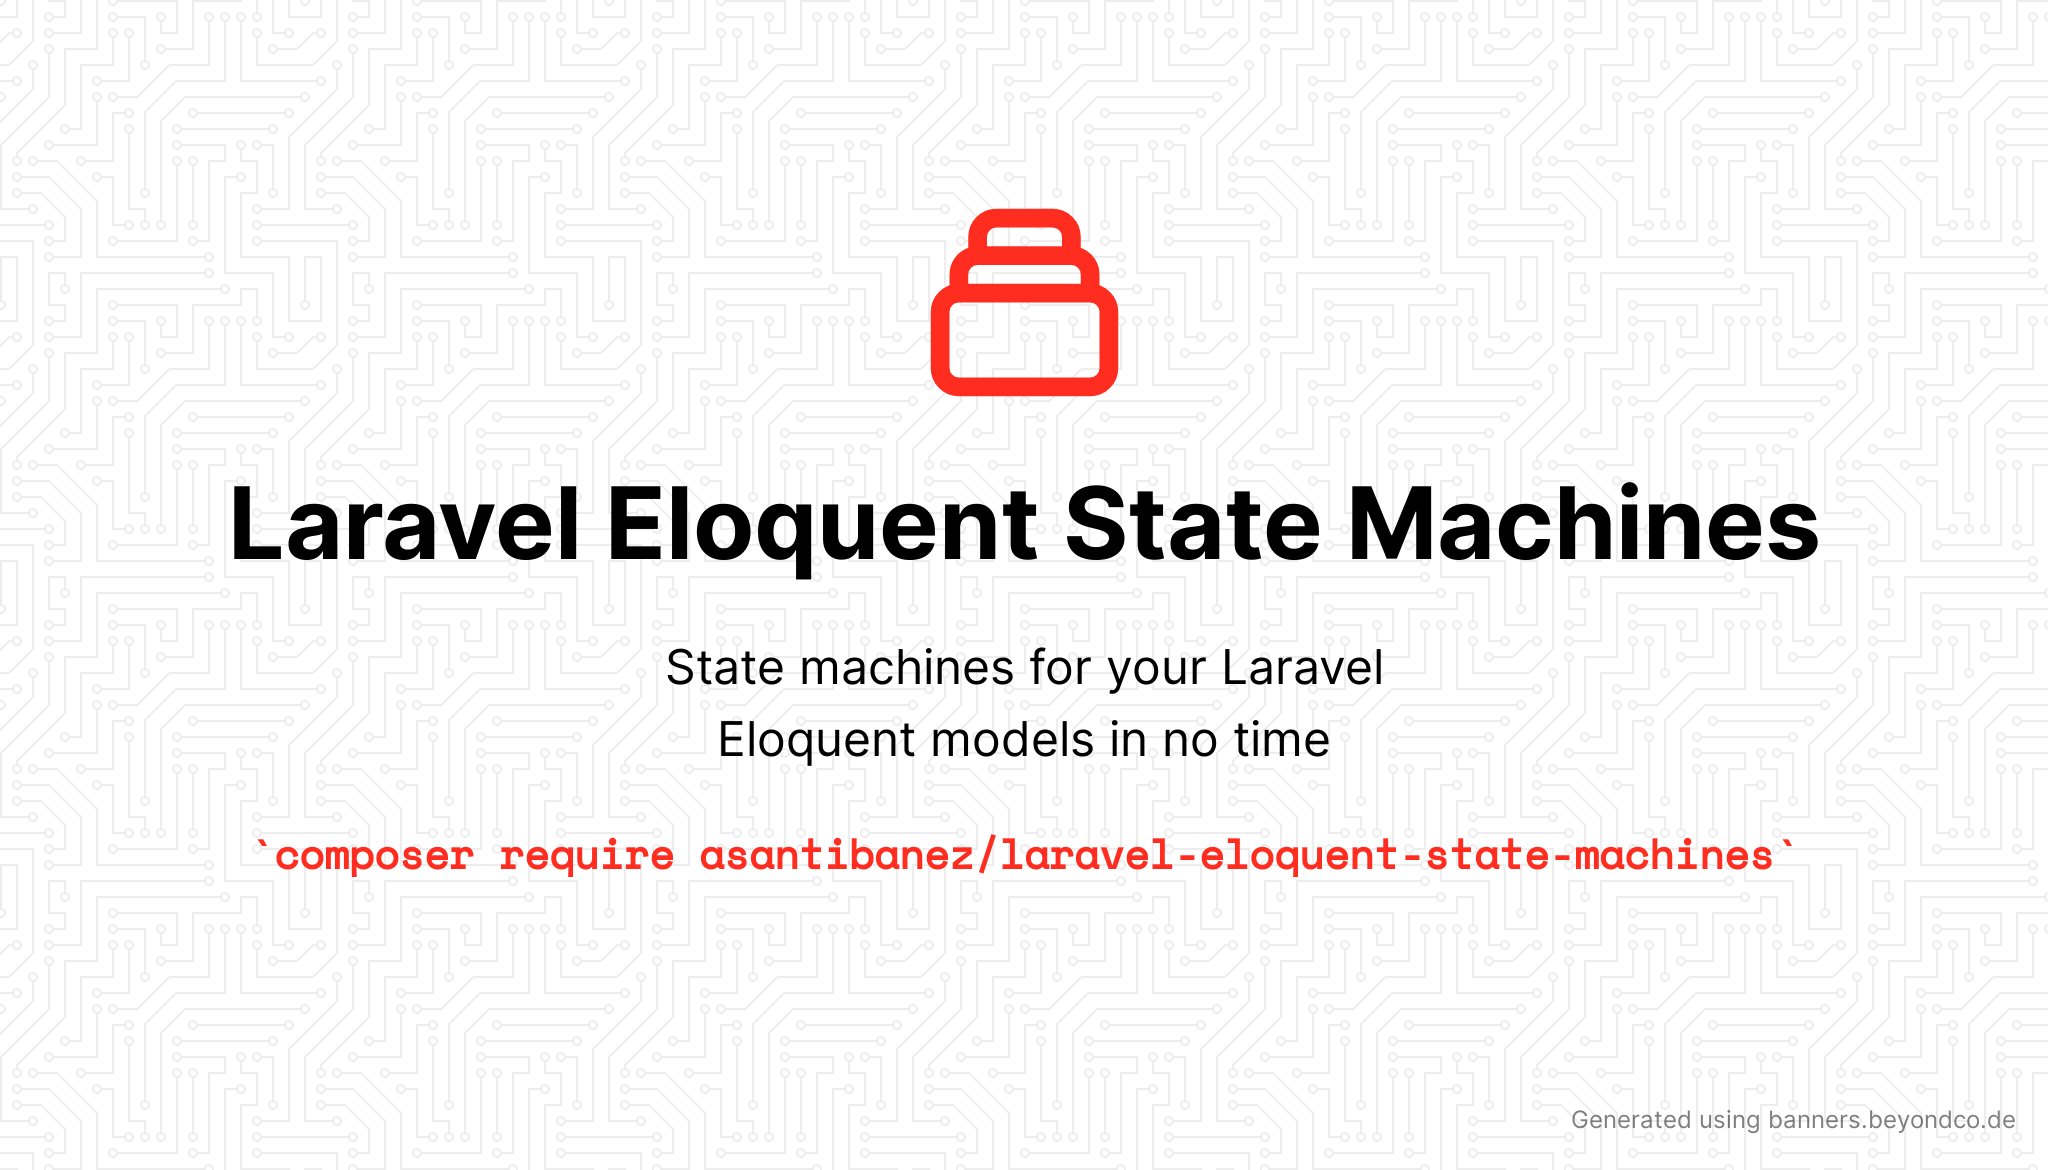
\includegraphics[width=0.7\textwidth]{assets/laravelstatemachines}
    \caption{Paquete de manejo de estados en Laravel}{Fuente: https://github.com/asantibanez/laravel-eloquent-state-machines}
    \label{fig:laravelstatemachines}
\end{figure}

De los tres paquetes anteriores, sin duda el de las máquinas de estados es el que más inspirará este proyecto. La funcionalidad es similar a la que se pretende, pero no es específica a los procesos administrativos y por lo tanto no brinda ciertas herramientas que podrían ser necesarias en los mismos, como el seguimiento, el cual podría ser implementado con la ayuda del segundo paquete mencionado.

\section{Planteamiento del Problema}

\label{problem_statement} Gobiernos de todo el mundo buscan digitalizar sus
procesos para facilitar la interacción con la población y aumentar la eficiencia
de los mismos, apuntando a lo que la CEPAL llama Gobiernos Digitales y Gobiernos
Inteligentes.

Dentro de todos los procesos administrativos la figura de trámite y el
seguimiento del mismo se encuentra siempre presente a todo nivel y suele ser
motivo o parte del motivo de la creación de muchos sistemas de software
gubernamentales.

El desarrollo de sistemas de software es un proceso largo que requiere por sí
mismo la toma de varias decisiones profesionales para brindar a los usuarios el
mejor producto en el menor tiempo posible y garantizando que se cumplan ciertos
requerimientos funcionales y no funcionales, implicando una gran complejidad que
sería limitante si no fuera por algunas buenas prácticas de desarrollo.

A menudo, los equipos de desarrollo, para evitar que la complejidad de los
sistemas sea excesiva, buscan herramientas de terceros que les permiten no
reinventar la rueda. Estas herramientas, llamadas paquetes de software, que
pueden ser librerías o incluso frameworks de desarrollo, ofrecen una serie de
ventajas a los proyectos de desarrollo, así como algunas limitaciones que, en la
mayoría de los casos, y dependiendo del proyecto, no son relevantes, pero
requieren la atención del equipo de profesionales.

Estas herramientas, que forman parte fundamental del desarrollo moderno, suelen
ser de código abierto, o al menos así se prefieren por muchos profesionales,
dadas sus ventajas de seguridad y versatilidad.

Es importante notar también que en algunos países se demanda o prefiere el uso
de software libre en el ámbito público. Tal es el caso de Bolivia, que en su
artículo 77 de la ley general de telecomunicaciones, tecnologías de información
y comunicación indica que se debe promover y priorizar el uso del mismo dentro
de los órganos ejecutivo, legislativo, judicial y electoral.

Por lo anteriormente descrito podemos encontrar una gran cantidad de tecnologías
abiertas usadas para el desarrollo de sistemas, como la librería Carbon de PHP,
el estándar EcmaScript o el popular framework de desarrollo Laravel, las cuales,
a pesar de proporcionar utilidades que facilitan la creación de proyectos
pequeños y medianos de software, no proporcionan de manera específica un marco
de trabajo confiable y específico para trabajar con los tan frecuentes trámites
administrativos y su seguimiento, obligando a los desarrolladores a reinventar
la rueda en cada proyecto de este tipo.

El caso que se toma para este proyecto, que es el sistema SIAI del
Viceministerio de Desarrollo Productivo, desarrollado por la empresa 2IES, tiene
un módulo de seguimiento de trámites realizado desde cero para el mismo y,
además de ser en el que se basará este proyecto y sobre el cual se aplicará para
medir el éxito del mismo, es un claro ejemplo de la necesidad de un paquete
reutilizable para la creación de módulos de trámites y seguimiento de trámites.

Otros sistemas, cuyo código fuente, se escapan al conocimiento del autor de este
documento, pero que se estima requirieron un desarrollo desde cero para su
módulo de trámites son:

\begin{itemize}
	\item Sistema de Matriculación de la UMSA

	\item Sistema para permisos de vidrios polarizados

	\item Sistema para permisos de circulación en pandemia

	\item Procedimiento para autorización de vidrios oscurecidos
\end{itemize}

\begin{figure}[h]
	\centering
	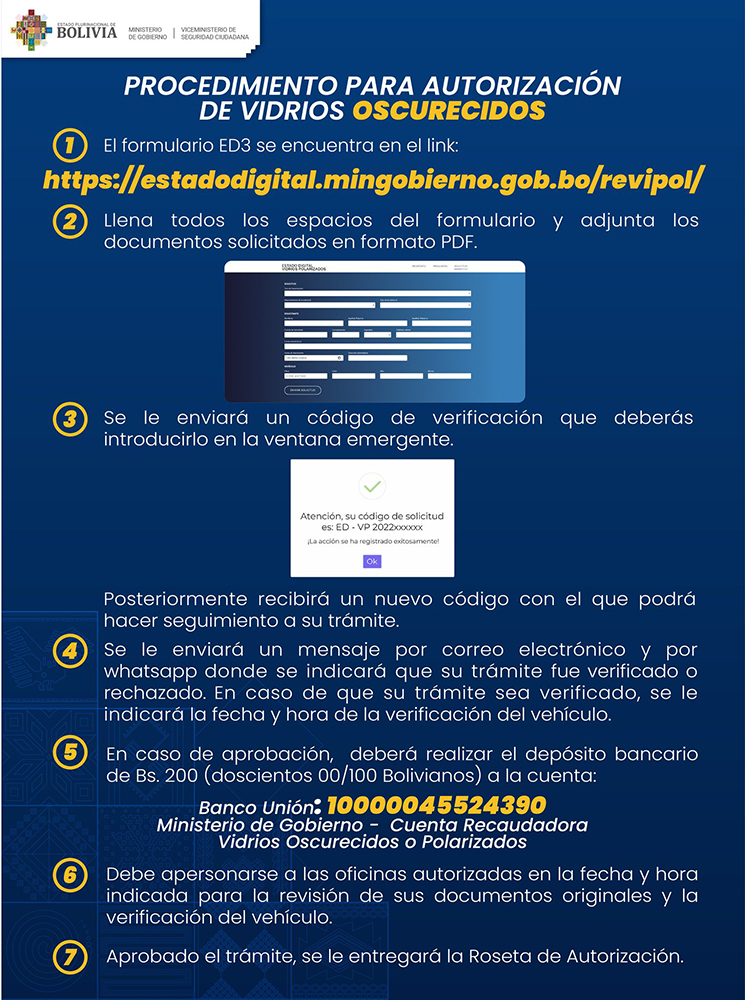
\includegraphics[width=0.6\textwidth]{assets/tramiteoscurecidos.jpg}
	\caption{Pasos del trámite para vidrios oscurecidos que se realizó en línea}
	\label{fig:polarized_procedure_steps}
\end{figure}

Entre los sistemas anteriormente expuestos, se hace énfasis en los sistemas
creados en época de pandemia, o el caso de los vidrios oscurecidos de la figura
\ref{fig:polarized_procedure_steps} , los cuales debían ser desarrollados con
premura dadas las circunstancias, lo cual puede ser facilitado con una librería
de software.

La carencia de una librería específica a los trámites y su seguimiento hacen
visibles varias desventajas:

\begin{itemize}
	\item Reinvención de la rueda en varios proyectos de características
		similares.

	\item Poca atención al detalle para un módulo de gran importancia.

	\item Tiempos de desarrollo mayores.

	\item Mayor coste.

	\item Sobre-ingeniería en proyectos pequeños.

	\item Menor adopción de sistemas digitales en el aparato público.

	\item Mayor susceptibilidad a desarrollos fallidos.

	\item Falta de características.

	\item Dificultad mayor en la redacción de la documentación.

	\item Poca presencia de proyectos open source bolivianos.
\end{itemize}

Actualmente existen librerías que ayudan con un concepto muy útil en el
seguimiento de trámites que son las máquinas de estados. Sin embargo, no son
específicas, son poco usadas y carecen de una buena documentación o facilidades
para el desarrollador.

Además, sistemas similares a los de seguimientos de trámite también existen en
el mercado, pero como productos cerrados y genéricos que no garantizan seguridad
para un sistema gubernamental y no pueden ser reutilizados por varios proyectos
de forma gratuita como es el caso de una librería de código abierto.

Por lo expuesto, se tiene una visión inicial que consiste en la premisa de que
cuando una funcionalidad es común en distintos sistemas, una solución viable y
común es la creación de una herramienta reutilizable de código abierto que ayude
en su implementación. Esto proporciona varias ventajas y se suscribe al
principio DRY \brackettext{Don't repeat yourself} y al primer principio SOLID
sobre la single responsibility.

Sin embargo, una librería open source acarrea varios desafíos en su realización,
muchos de ellos académicos, de los cuales a continuación se listan algunos:

\begin{itemize}

	\item Elección de un entorno sobre el cual aplicar este proyecto: Una
		librería puede estar limitada a un lenguaje de programación o incluso a
		un marco de desarrollo. Esta decisión es importante tomarla al inicio
		del proyecto.

	\item Metodología de desarrollo: Adoptar una buena metodología es importante
		en una librería, ya que ésta será utilizada por muchos proyectos que
		confiaran en la misma. Además, al ser open source, se espera que de
		tener éxito la misma siga mejorando.

	\item Arquitectura de Software: Este es un tema muy someramente estudiado
		durante el transcurso de la carrera de ingeniería Electrónica de la
		UMSA, pero es muy necesario para tomar las mejores decisiones en el
		desarrollo de un sistema.

	\item Documentación: Escribir la documentación de una librería que se espera
		sea utilizada por muchas personas es de mayor relevancia. Se requiere un
		buen lenguaje técnico y habilidades de redacción, pero a la vez la
		capacidad para que lo descrito sea fácil de entender por la mayor
		cantidad de personas.

	\item Knowhow open source: Se cuenta con muy poco conocimiento del
		desarrollo de software libre en el contexto local y mucho menos de
		sistemas con éxito.

	\item Versionado: Cualquier proyecto de software moderno requiere el uso de
		sistemas de versionado, pero en un proyecto de código abierto esto es
		especialmente importante para permitir colaboraciones externas.

	\item Buenas prácticas de desarrollo y uso de patrones de diseño: Para tener
		una buena librería existen libros de recomendaciones y patrones que
		pueden ser empleados, además de experiencias compartidas en internet por
		distintos desarrolladores.  Las mismas pueden potenciar un proyecto y
		son importantes de aprender.

	\item Infraestructura y escalabilidad: La librería debe ser pensada para
		poder ser desplegada en sistemas grandes y poder ser escalable. El tema
		de escalabilidad es en sí mismo un campo de estudio dentro del
		despliegue de sistemas.

	\item Testabilidad: Los proyectos de software moderno tienen como proceso
		importante el del testing, el cual permite realizar desarrollos que cumplan con
		lo que se desea en su diseño y que no hagan algo distinto \parencite{myersArtSoftwareTesting2012}.
		Sin embargo, el campo del testing no es ni minimamente explorado en
		instituciones universitarias, a pesar de su importancia.
\end{itemize}
\section{Objetivos}

\section{Justificación}
La solución propuesta tiene 3 pilares importantes que la componen y muestran relevancia cada una por su cuenta:

\begin{itemize}
    \item La figura del paquete de software reutilizable.
    \item La figura del trámite en instancias gubernamentales y su modernización.
    \item El desarrollo de software libre.
\end{itemize}

De acuerdo a esto podemos ver la importancia de esta solución en distintos ámbitos:

\subsection{Tecnológico}
La creación de un paquete de software reutilizable para la creación y
seguimiento de trámites ayuda en el proceso de digitalización de uno de los
procedimientos más comunes en el ámbito público, brinda a los gobiernos la
posibilidad de aprovechar de mejor manera los datos resultantes de un trámite y
dan a la población herramientas que hacen más fáciles sus vidas.

Al usar máquinas de estados finitas logramos el aprovechamiento del conocimiento
en sistemas secuenciales digitales dentro del ámbito de sistemas de software
para lograr una abstracción del trámite.

El paquete no sólo facilitará la implementación de sistemas de software con
módulos de trámites, sino que de forma más directa simplificará la tarea de los
desarrolladores, siendo una pieza tecnológica dentro de proyectos más amplios.

\subsection{Económico}
El software reutilizable de código abierto suele se aprovechado hoy en día con el objetivo de
disminuir costos en la producción de sistemas gracias a su naturaleza de
comunidad y lo demandado de su funcionalidad.

De no existir el software reutilizable se deben invertir recursos para cada
proyecto que requiera la misma funcionalidad. Recursos que, de usar un paquete
de software, podrían conservarse, siendo que una parte del desarrollo ya estaría
implementada. Existen excepciones a este caso en proyectos con necesidades muy
específicas, pero en la mayoría de proyectos, una librería o framework bien
implementado son esenciales para disminuir costos de producción.

\subsection{Académico}
Los proyectos de software libre a nivel regional y a nivel universidad son
realmente escasos y al momento de redacción de este documento se desconoce de
algún caso de éxito en la carrera de Ingeniería Electrónica de la UMSA.

Es por eso que este proyecto busca ser un punto de partida hacia la realización
de más proyectos del mismo tipo, es decir, de software libre reutilizable. Todo
esto a partir de esta travesía que a modo de ejemplo busca inspirar a más
estudiantes de la carrera.

\subsection{Político}
La realización de este proyecto no sólo se alinea con la necesidad de los
distintos gobiernos del mundo de digitalizar sus procesos administrativos - como
se puede constatar en Bolivia por el decreto xxx donde se solicita a las
distintas instituciones gubernamentales la realización de planes hacia un
gobierno electrónico -, sino además apunta a la preferencia que los gobiernos
tienen por el software libre, como se describe en el artículo xx de la ley xx.

\subsection{Social}
Los trámites son un dolor de cabeza para gran parte de la sociedad. Los
gobiernos hacen el intento por digitalizar los mismos y así aliviar a la
población, pero la existencia de herramientas reutilizables pueden acelerar
drásticamente este proceso. Se espera que más y más trámites sean digitalizados
en tanto más fácil sea hacerlo. De esta manera los distintos actores de la
sociedad podrán aprovechar las bondades de las tecnologías de la información.

La digitalización de trámites, que sería facilitada por este proyecto, mejora
además los mecanismos por los cuales la sociedad participa del gobierno. Impulsa
la apertura de la información de los gobiernos hacia la gente y se adecúa a las
nuevas necesidades de las personas.
\section{Alcances y Limitaciones}

\section{Descripción de la Solución Propuesta}
Dada la problemática expuesta en la sección \ref{problem_statement}, en la que
se describe de manera breve el enfoque que se le piensa brindar, en esta sección
se trata de describir la primera aproximación a su solución de forma detallada.

Sin duda, la realización de una herramienta de software libre reutilizable para
la implementación de trámites y su correspondiente seguimiento a nivel de
backend tiene muchas ventajas, pero su realización no es del todo trivial y
demanda que se conceptualice en un modelo medianamente robusto, con metodologías
claras y descripciones escuetas.

Cuando uno piensa en trámites, usualmente piensa en burocracia, en largas filas,
una obligación muchas veces irrenunciable y una lista interminable de pasos a
seguir. Según la Real Academia de la Lengua Española, se define como \say{Cada
	uno de los pasos y diligencias que hay que recorrer en un asunto hasta su
	conclusión} \parencite{asaleDiccionarioLenguaEspanola}.

Si bien las definiciones de trámite son escasas y algunas pueden tratar su
semántica desde una perspectiva más funcional, es indudable que un trámite es un
procedimiento que consta de uno o más pasos a seguir. De este modo, se puede
vislumbrar una manera casi obvia de modelarlo usando conceptos de teoría
computacional, de matemáticas discretas o circuitos secuenciales. Esto es,
usando máquinas de estado finitas.

Este enfoque no es precisamente nuevo y ya se puede ver en una aproximación al
modelado en software de distintos trámites de la división de gestiones,
admisiones y registros de la UMSA, donde se emplearon máquinas de Turing que a
efectos prácticos se aproximan más a máquinas de estado finitas
\parencite{nachoSISTEMACONTROLTRAMITES2007}, como se puede ver en la figura
\ref{fig:nachocarreraparalela}.

\begin{figure}
	\centering
	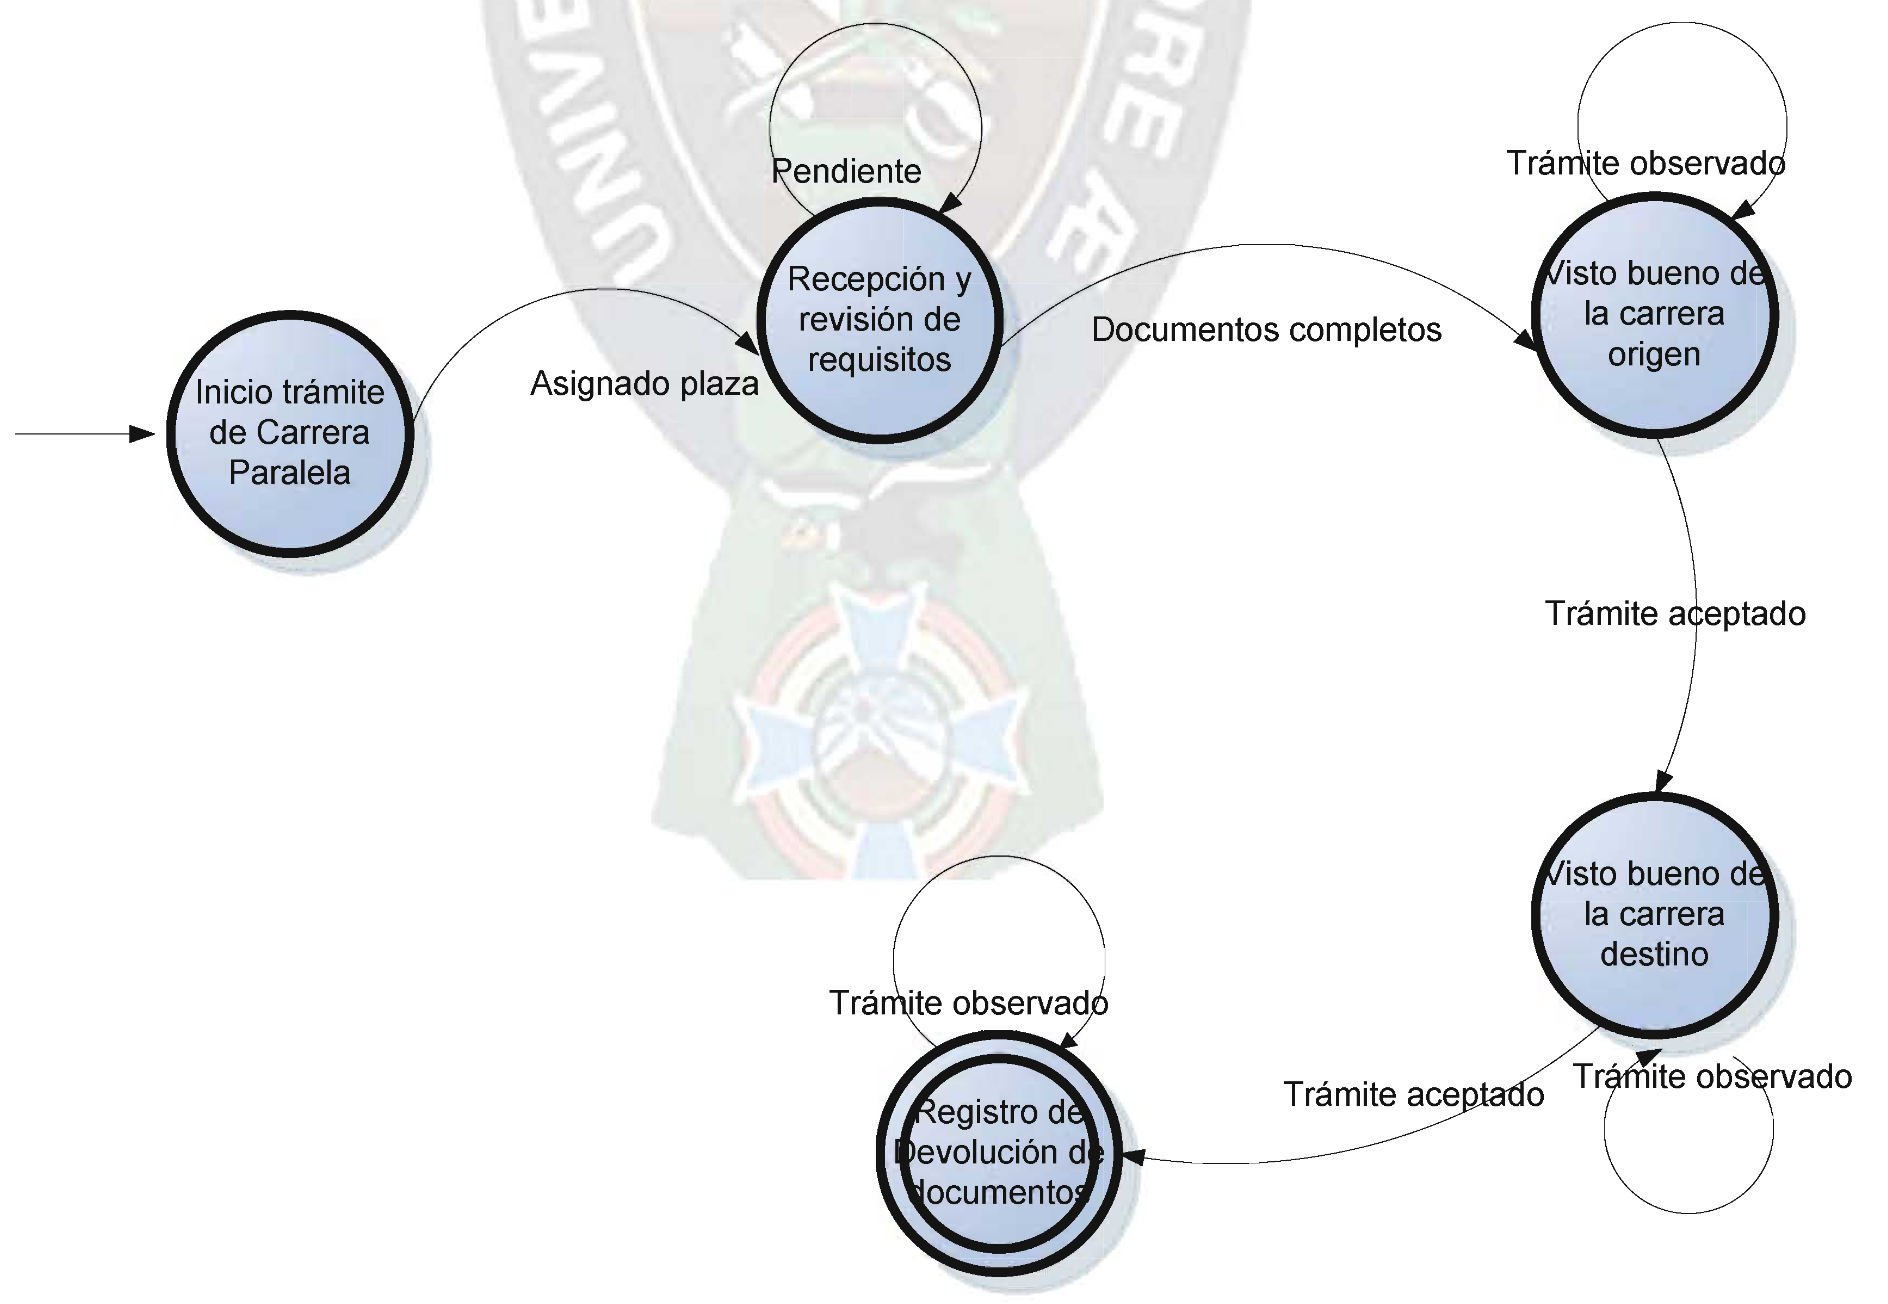
\includegraphics[width=0.7\textwidth]{assets/carreraparalelanacho}
	\caption{Diagrama de una máquina de Turing para carreras paralelas
		desarrollada en \cite{nachoSISTEMACONTROLTRAMITES2007}}
	\label{fig:nachocarreraparalela}
\end{figure}

Desde luego, las máquinas de estados finitas parecen ser una manera sencilla de
modelar los procesos de trámite a nivel de software, principalmente por su
paralelismo con los pasos y sus respectivas transiciones, asemejándose a un
procedimiento administrativo, como se puede evidenciar en la definición
matemática de este autómata:

\begin{definition}[Máquina de Estados Finita]
	Una máquina de estados es un conjunto de 5 elementos $M=(S,I,O,v,w)$, donde
	$S$ representa a la colección de estados de $M$; $I$ representa al alfabeto
	de entradas para M; O es el alfabeto de salidas de M; $v:SxI->S$ es la
	función del siguiente estado; y $w:SxI->O$ es la función de salida
	\parencite{grimaldiDiscreteCombinatorialMathematics1998}.
\end{definition}

Este paralelismo es más notorio en un diagrama de estados como el que se muestra
en la figura \ref{fig:states}, donde tenemos los estados de $S = (s_{0}, s_{1},
	s_{2}, s_{3}, s_{4}, s_{5}, s_{error})$ y algunas transiciones entre los mismos,
cada una con sus correspondientes entradas ($\iota_{mn}$) y salidas ($o_{mn}$).
Las transiciones restantes se omiten porque apuntan a un mismo estado de error
del trámite ($s_{error}$).

\begin{figure}[ht]
	\centering
	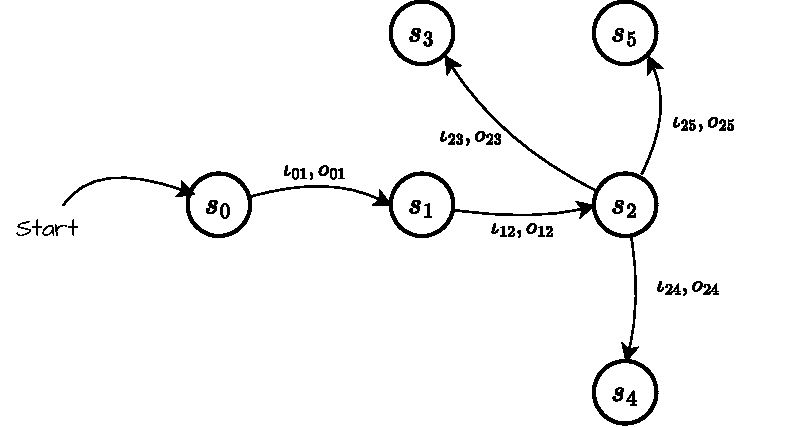
\includegraphics[width=0.8\textwidth]{assets/statediagramexample}
	\caption{Diagrama de estados finitos con salidas}
	\label{fig:states}
\end{figure}

En la figura \ref{fig:states_procedure} podemos ver el mismo diagrama, pero
simplificado y usando un lenguaje cercano a la naturaleza de los procedimientos
administrativos de forma adrede para hacer más obvia la relación descrita.
Nótese que se usan para los estados nombres cortos y no totalmente detallados
para fines prácticos de ilustración. En un sistema real se esperan definiciones
claras que reflejen la totalidad del trámite implementado.

\begin{figure}[ht]
	\centering
	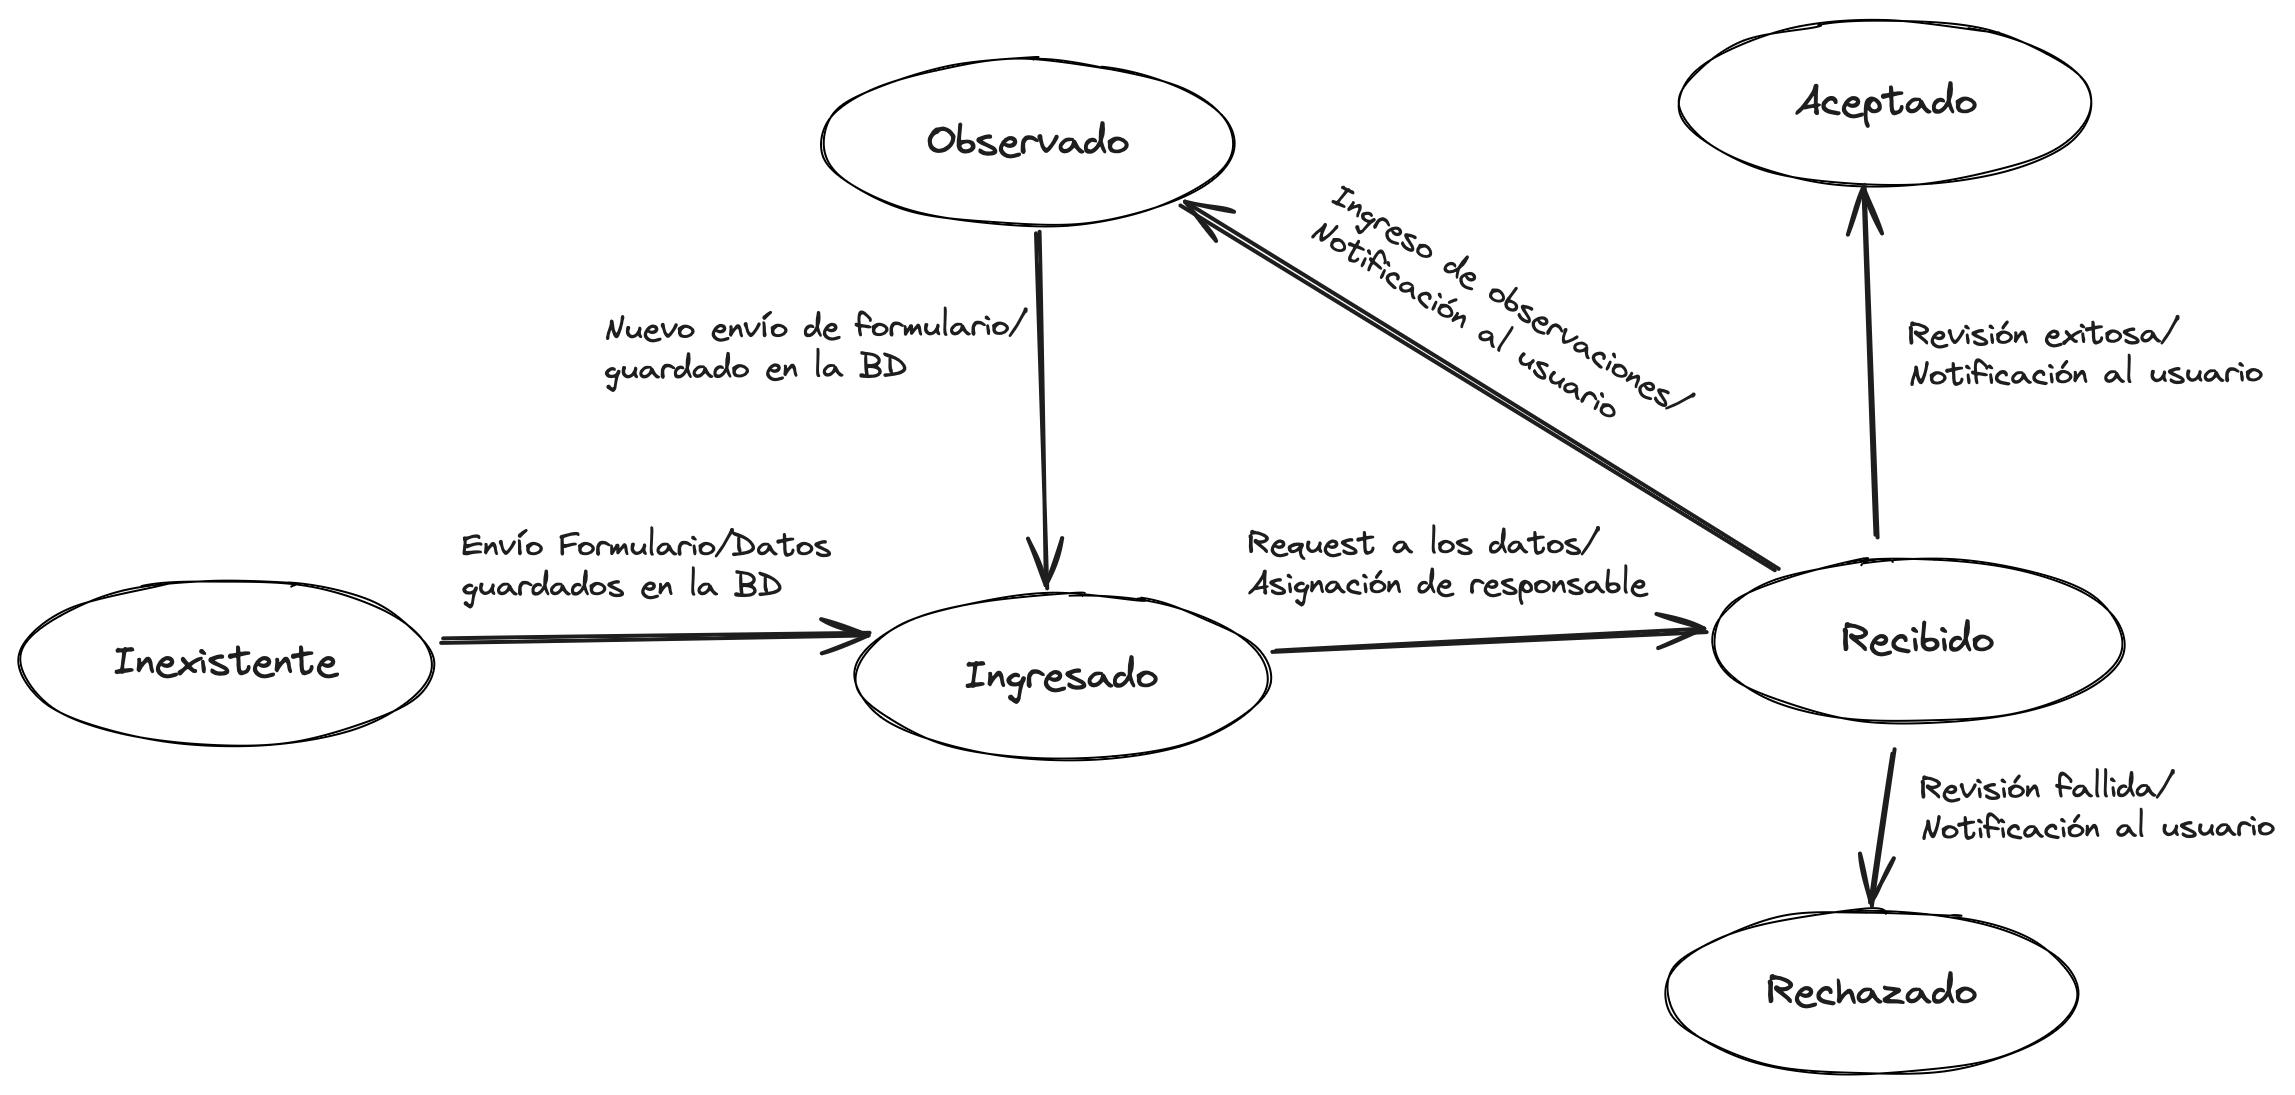
\includegraphics[width=0.8\textwidth]{assets/stateprocedureexample}
	\caption{Diagrama de estados simplificado para un trámite}
	\label{fig:states_procedure}
\end{figure}

Se plantea utilizar este enfoque del uso de autómatas, como también son llamadas
las máquinas de estado en contextos de teoría computacional, pero con ciertos
lineamientos conceptuales que guíen al usuario de esta solución, que
inicialmente serían:

\begin{itemize}
	\item Descripción detallada de los estados, compuesta mínimamente por un
	      nombre único, una descripción, el sujeto cuya perspectiva se usa para la
	      descripción y su visibilidad.

	\item Preferencia del autómata de Moore sobre el autómata de Mealy. Los
	      autómatas de Mealy son una simplificación en número de estados a partir
	      de los autómatas de Moore, con estados que en las aplicaciones
	      originales del concepto podían ser considerados innecesarios
	      \parencite{mealyMethodSynthesizingSequential1955}.  Si bien en muchas
	      aplicaciones es lo deseado, en temas de auditoría se prefiere tener la
	      mayor cantidad de información relevante, por lo que sin restringir el
	      uso de máquinas de Mealy, se priorizará el uso de máquinas de Moore.

	\item Respecto al anterior punto, incluso si el usuario usa Mealy en lugar
	      de Moore, se recomienda la definición de tantos estados como sean
	      posibles.

	      % TODO: Aquí irían las definiciones de inputs, outputs, etc como lo tengo
	      % descrito en el Obsidian
\end{itemize}

Como parte de la solución propuesta, se debe entender que los lineamientos
conceptuales son muy importantes, ya que este proyecto no será solamente de
código abierto, sino además de concepto abierto, es decir, estas ideas se pueden
aplicar en otros entornos distintos al que se elegirá para esta solución
\cite[439]{sommervilleSoftwareEngineering2016}, el cual se detalla más adelante.

Cualquier implementación de software implica una toma detallada de
requerimientos sobre la cual trabajar. Quizá una desventaja del software libre
en la práctica es que las metodologías no son aplicadas correctamente, los
programadores definen los requerimientos y no hay objetivos medibles
\cite[Tabla~1]{aberdourAchievingQualityOpenSource2007}; esto debido a que no
existen las figuras de cliente, inversión y beneficio económico, que
precisamente son la fuente de los requerimientos más importantes para el
proyecto.

Por esto mismo, para la solución planteada se aprovechará el ya existente
proyecto SIAI (Sistema Integral Ambiental Industrial) del Viceministerio de
Desarrollo Productivo, desarrollado por la empresa 2IES y en el cual, el autor
de este documento, tuvo participación. Este sistema contempla requerimientos
comunes en la realización de trámites gubernamentales y será una guía para la
implementación actual.

Evidentemente, al ser un proyecto de código libre y al pretender dejar su
desarrollo abierto desde el día 1 en Github, sería un despropósito no aprovechar
y/o buscar más proyectos similares que puedan enriquecer el desarrollo actual.

El sistema SIAI, que será empleado como referencia, tendrá además otro papel
importante en este proyecto, siendo el producto del mismo utilizado en una
implementación de un fork del mencionado software para demostrar la usabilidad
del paquete.

Esto nos obliga a tomar una decisión a priori sobre el desarrollo del producto
que se propone como solución y es que, como cualquier otro paquete de software,
su implementación suele estar restringida a alguna tecnología existente
\cite[444]{sommervilleSoftwareEngineering2016}.  Dada la popularidad del
framework Laravel de PHP y a que el sistema SIAI está desarrollado usando estas
tecnologías se procederá a la creación de un paquete, precisamente, de Laravel.

La solución, al ser un paquete de software, contará no solamente con las ideas y
marcos de trabajo descritos anteriormente, sino que además se piensa brinde
herramientas que ayuden al proceso de trámites, como por ejemplo:

\begin{itemize}
	\item Generación de códigos de trámite.

	\item Generación de códigos de verificación de correos (Que si bien hay
	      alternativas para lo mismo, se facilitará el uso desde el paquete).

	\item Funcionalidad de notificaciones.

	\item Límites de tiempo asignables a los estados de trámite.

	\item Funcionalidad de persistencia de historial de estados incorporada.

	\item Funciones de recuperación de historia de trámite para seguimiento.

	\item Niveles de visibilidad de trámites para seguimiento.

	\item Mecanismos para dificultar el entorpecimiento de un trámite y
	      facilitar la identificación de responsables.

	\item Interfaz sencilla para cambio de estados de una máquina (trámite).
\end{itemize}

Para concluir esta aproximación a la solución a realizar, quedan dos puntos
importantes a tocar, uno de ellos opcional a la fecha de redacción de este
documento, y es acerca de la naturaleza FLOSS o FOSS de este proyecto.

Para que un proyecto de software sea considerado de software libre debe cumplir
con 4 libertades esenciales \cite{QueEsSoftware}:

\begin{itemize}
	\item La libertad de ejecutar el programa como se desee, con cualquier
	      propósito (libertad 0).

	\item La libertad de estudiar cómo funciona el programa, y cambiarlo para
	      que haga lo que se desee (libertad 1). El acceso al código fuente es una
	      condición necesaria para ello.

	\item La libertad de redistribuir copias para ayudar a otros (libertad 2).

	\item La libertad de distribuir copias de sus versiones modificadas a
	      terceros (libertad 3). Esto le permite ofrecer a toda la comunidad la
	      oportunidad de beneficiarse de las modificaciones. El acceso al código
	      fuente es una condición necesaria para ello.
\end{itemize}

Esto debe ser claramente definido en un documento de licencia de Software que se
encuentre junto al código fuente. Existen varias licencias que cumplen con los
lineamientos antes señalados y son aprobados por la FSF (Free Software
Foundation) \cite{VariousLicensesComments}.

Si bien la licencia predilecta del Software Libre es la GNU-GPL, de la cual
existe incluso una versión boliviana llamada LPG-Bolivia
\cite{cayoLPGBoliviaADSIB}, puede ser demasiado restrictiva para quien quiera
usar los resultados de este proyecto. Por esto mismo se piensa licenciar no sólo
el software sino también los documentos de proyecto asociados bajo alguna
licencia similar a la del MIT \cite{MITLicense2006}, que brinda la posibilidad
de generar software no libre a partir de software libre y es ampliamente usado
por varios proyectos Open Source.

Un proyecto de software libre suele ser distribuido en la red y suele tener
alguna denominación distintiva. Dada la naturaleza de los trámites, que consiste
en una secuencia de pasos se piensa bautizar al paquete resultante de este
proyecto como \say{Tunkunia}.
%% \section{Presupuesto Tentativo}

\section{Temario}

Para el temario del documento final de proyecto se considerará una estructura que describa bien la naturaleza del proyecto y que además se adecúe a este que, después de todo, será un producto de software.

De acuerdo a la ingeniería de software, el software tiene un ciclo de vida o un \say{proceso del software}, el cual se modela de acuerdo a la metodología de desarrollo sobre la cual se realice. Sin embargo, varios autores concuerdan en que existen ciertas etapas estructurales ajenas a cualquier metodología. Según Pressman \cite[13]{pressmanSoftwareEngineeringPractitioner2010}, estas etapas serían:

\begin{itemize}
    \item Comunicación.
    \item Planeación.
    \item Modelado.
    \item Construcción.
    \item despliegue.
\end{itemize}

Por su lado, Sommerville las simplifica en 4 etapas:

\begin{itemize}
    \item Software Specification.
    \item Software Development.
    \item Software Validation.
    \item Software Evolution.
\end{itemize}

El temario del documento final del proyecto obedecerá entonces a esta definiciones del proceso de software para no depender de la metodología usada.

Nótese, sin embargo, que este temario es tentativo, lo cual quiere decir que pueden surgir cambios durante la realización del proyecto.

\begin{itemize}
    \item Presentación
    \item Agradecimientos
    \item Resumen
    \item Índice
    \item Glosario
\end{itemize}

\begin{syllabus}
    \item \textbf{Generalidades del proyecto:} Describirá los antecedentes del proyecto, así como la problemática que se ha identificado, para la cual se plantea una solución a través del objetivo. De igual modo se hará referencia a la justificación del proyecto y los alcances y límites que se plantearon durante su gestación.
    \item Revisión de la literatura
    \item Definición de requerimientos
    \item Modelado y conceptualización
    \item Implementación
    \item Pruebas de Validación
    \item Despliegue
    \item Integración en el SIAI
    \item Resultados y conclusiones
\end{syllabus}

\begin{itemize}
    \item Bibliografía y Referencias
    \item Anexos
\end{itemize}
\section{Cronograma}
\printbibliography
\addcontentsline{toc}{section}{Bibliografía y Referencias}
\end{document}